\documentclass[a4paper]{article} 
\addtolength{\hoffset}{-2.25cm}
\addtolength{\textwidth}{4.5cm}
\addtolength{\voffset}{-3.25cm}
\addtolength{\textheight}{5cm}
\setlength{\parskip}{0pt}
\setlength{\parindent}{0in}

%----------------------------------------------------------------------------------------
%	PACKAGES AND OTHER DOCUMENT CONFIGURATIONS
%----------------------------------------------------------------------------------------

\usepackage{blindtext} % Package to generate dummy text
\usepackage{charter} % Use the Charter font
\usepackage[utf8]{inputenc} % Use UTF-8 encoding
\usepackage{microtype} % Slightly tweak font spacing for aesthetics
\usepackage[english, ngerman]{babel} % Language hyphenation and typographical rules
\usepackage{amsthm, amsmath, amssymb} % Mathematical typesetting
\usepackage{float} % Improved interface for floating objects
\usepackage[final, colorlinks = true, 
            linkcolor = black, 
            citecolor = black]{hyperref} % For hyperlinks in the PDF
\usepackage{graphicx, multicol} % Enhanced support for graphics
\usepackage{xcolor} % Driver-independent color extensions
\usepackage{marvosym, wasysym} % More symbols
\usepackage{rotating} % Rotation tools
\usepackage{censor} % Facilities for controlling restricted text
\usepackage{listings, style/lstlisting} % Environment for non-formatted code, !uses style file!
\usepackage{pseudocode} % Environment for specifying algorithms in a natural way
\usepackage{style/avm} % Environment for f-structures, !uses style file!
\usepackage{booktabs} % Enhances quality of tables
\usepackage{tikz-qtree} % Easy tree drawing tool
\tikzset{every tree node/.style={align=center,anchor=north},
         level distance=2cm} % Configuration for q-trees
\usepackage{style/btree} % Configuration for b-trees and b+-trees, !uses style file!
\usepackage[backend=biber,style=numeric,
            sorting=nyt]{biblatex} % Complete reimplementation of bibliographic facilities
\addbibresource{ecl.bib}
\usepackage{csquotes} % Context sensitive quotation facilities
\usepackage[yyyymmdd]{datetime} % Uses YEAR-MONTH-DAY format for dates
\renewcommand{\dateseparator}{-} % Sets dateseparator to '-'
\usepackage{fancyhdr} % Headers and footers
\pagestyle{fancy} % All pages have headers and footers
\fancyhead{}\renewcommand{\headrulewidth}{0pt} % Blank out the default header
\fancyfoot[L]{} % Custom footer text
\fancyfoot[C]{} % Custom footer text
\fancyfoot[R]{\thepage} % Custom footer text
\newcommand{\note}[1]{\marginpar{\scriptsize \textcolor{red}{#1}}} % Enables comments in red on margin

%----------------------------------------------------------------------------------------

\begin{document}

%-------------------------------
%	TITLE SECTION
%-------------------------------

\fancyhead[C]{}
\hrule \medskip % Upper rule
\begin{minipage}{0.295\textwidth} 
\raggedright
\footnotesize
\textbf{Jaime Andres Torres Bermejo} \hfill\\   
202014866\hfill\\
andrestbermejoj@gmail.com\hfill\\

\textbf{Santiago Latorre Munar}\hfill\\
202111851\hfill\\
s.latorre@uniandes.edu.co

\textbf{Santiago Forero Gutiérrez} \hfill\\
202111446 \hfill\\
s.forerog2@uniandes.edu.co

\end{minipage}
\begin{minipage}{0.4\textwidth} 
\centering 
\large 
Caso 2\\ 
\normalsize 
Infraestructura Computacional\\ 
\end{minipage}
\begin{minipage}{0.295\textwidth} 
\raggedleft
\today\hfill\\
\end{minipage}
\medskip\hrule 
\bigskip

%-------------------------------
%	CONTENIDO
%-------------------------------
\section{Detalles de implementación}
\subsection{Modo 1}
Para lograr generar referencias de página en primer lugar se define una
posición inicial en páginas y desplazamiento para cada una de las 3 
matrices dependiendo del tamaño del entero, el tamaño de una página y 
el tamaño de la matriz. Una vez guardadas en distintas variables la 
página y desplazamiento inicial de cada matriz se inicia un ciclo para 
calcular la posición de cada entero de cada matriz. Para lograr esto 
se itera con un doble ciclo cada posición de las matrices (pues 
tienen mismo número de filas y columnas de modo que las posiciones 
coinciden). Para cada posición y para cada una de las 3 matrices se 
guarda en un String (que posteriormente se transformara en un archivo) 
la página y desplazamiento actual del entero de la posición actual de 
cada matriz. Es decir que por cada ciclo se almacena la posición 
equivalente de las tres matrices (pues así se calcula la suma). 
Posteriormente se actualiza la página y desplazamiento actual de cada 
matriz usando divisiones enteras y residuos. Para actualizar la página 
se le suma a la variable “el valor de sumar el desplazamiento actual y 
el tamaño de entero, dividido en una división entera por el tamaño de 
una página”. De forma que si la suma del desplazamiento actual y el 
tamaño de entero es menor al tamaño de página, la página permanece 
igual; y si es mayor, se aumenta en una posición la página. Respecto al 
desplazamiento se realiza la misma operación, pero en lugar de sumar a 
la variable se realiza una asignación y en lugar de hacer división 
entera se realiza la operación con módulo. De forma que si la suma del 
desplazamiento actual y el tamaño de entero es menor al tamaño de 
página, el desplazamiento se le suma el tamaño de entero; y si es 
mayor, se vuelve a iniciar en 0. Finalmente se trasforma esto a un 
archivo.

\subsection{Modo 2}
\subsubsection{Algoritmo de Envejecimiento.}
Con respecto al algoritmo de envejecimiento, este se encuentra localizado
en el Manejador, principalmente con el fin de poder acceder a la tabla de 
páginas de forma relativamente sencilla, cambiando valores como la edad binaria
de la página o el booleano que indica en memoria principal si se encuentra
o no. Esto reduce el tiempo de ejecución de la operación, lo cuál es importante
cuando consideramos que esta es una operación realizada varias veces por segundo.

Las condiciones y parámetros de las páginas estan definidos en la clase 'Página',
por lo que los 2 algoritmos principales del proceso de envejecimiento pueden
consultar una misma estructura y hacer cambios acordemente. El primer algoritmo
itera sobre la tabla de páginas, haciendo operaciones binarias sobre el int que
representa la edad de la página, mientras que el otro selecciona la página de
menor edad.

\section{Gráficos de ejecución}
\subsection{Prueba 1}
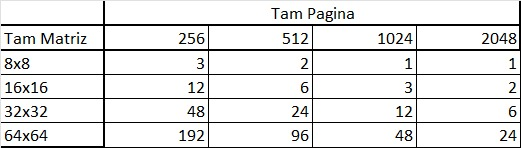
\includegraphics{1-1.jpeg}
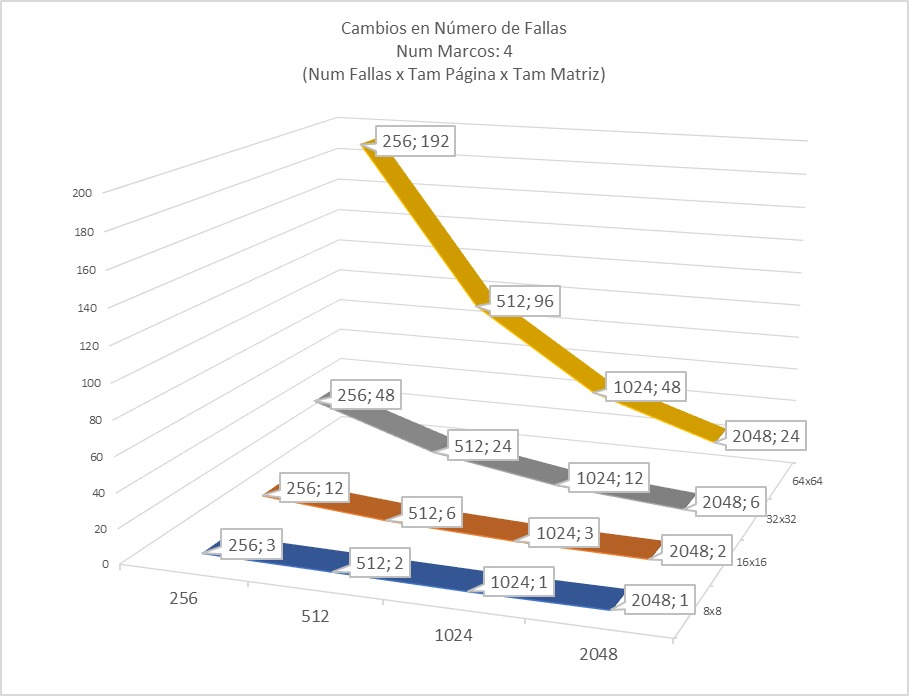
\includegraphics[scale=0.55]{1-2.jpeg}

\subsection{Prueba 2}
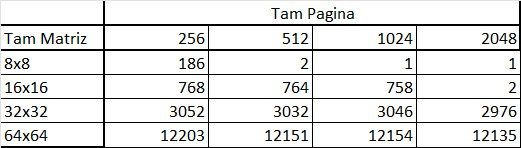
\includegraphics{2-1.jpeg}
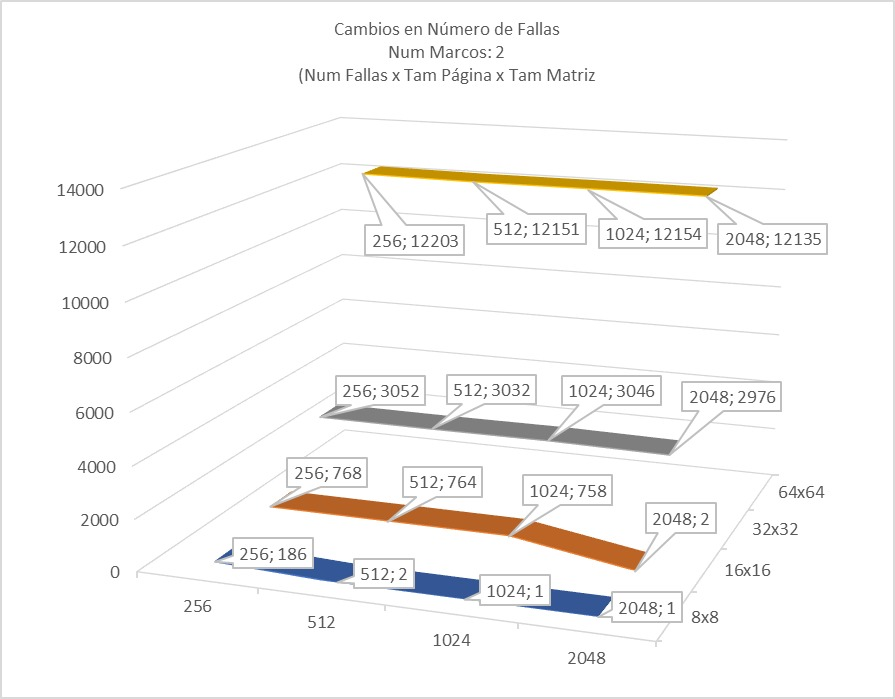
\includegraphics[scale=0.55]{2-2.jpeg}


%-------------------------------
\section{Preguntas realizadas.}
\subsection{¿Cómo varía el número de fallas de página si el algoritmo 
estudiado es el de multiplicación de matrices?}
La suma es una operación cuyo resultado generalmente no excede el 
tamaño de los sumandos, es decir, no requiere de una mayor cantidad de 
bits para ser representado en su forma binaria. Teniendo esto en cuenta 
y considerando que en el algoritmo solo se estudiaron tamaños de entero 
inferiores al tamaño de una página, se puede afirmar que para cargar los 
tres números de la suma (cada uno proveniente de su respectiva matriz) 
se requiere de máximo tres marcos de página. Por otro lado, dada la 
naturaleza de la multiplicación, es muchísimo más probable que el 
resultado adquiera un valor superior al de los factores, de manera que, 
en las mismas condiciones de la suma, será necesaria más de una página 
para almacenar este valor en su totalidad. Esto ya que para multiplicar 
matrices se tendría que realizar un producto punto para cada posición 
de la matriz resultado (recordar la fórmula de producto punto):

\begin{center}
    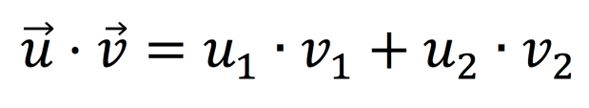
\includegraphics[scale=0.5]{prod_p.jpeg}    
\end{center}


Y, además, este calculo se realiza sobre la fila de una matriz y la columna de la otra, de forma que sería probable que se deban usar más páginas para guardar los cálculos parciales. Habiendo comprendido como se desenvuelven ambos algoritmos al cargarse en memoria virtual, llega el momento de revisar qué sucede cuando se quieren cargar a memoria real, lugar donde suceden las fallas de página: como ya se ha comprobado que en promedio una operación de multiplicación requiere de más páginas que una de suma, también necesitará de más marcos de página para cargarse en memoria real. Como resultado, se producirá una mayor cantidad de fallas al ser necesario reemplazar más frecuentemente las páginas para poder cargar los números que se requieran.



\end{document}
